\subsection*{High Level Data Flow Diagram}

\begin{center}
  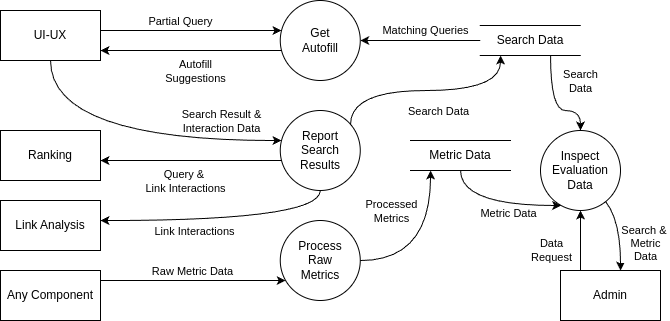
\includegraphics[scale=0.65]{DFDs/HighLevelDFD.drawio.png}
\end{center}

\subsection*{Architectural Divisions (APIs)}

\subsubsection*{Outgoing Calls}
These are the functions which we will call for other components to take action on.

\medskip

\textbf{Function:} \verb|sendRankingInteractions():|

\smallskip

\textbf{Destination Component:} Ranking

\smallskip

\textbf{Example Sent Data:} \begin{verbatim}
  {
    "processed_query": "Rensselaer Polytechnic Institute Professors",
    "links_ignored": [
      "link1.com",
      "link2.com"
    ],
    "link_clicked": "magical.awesome.link.com"
  },
\end{verbatim}

\smallskip

\textbf{Side Effects:} The Ranking algorithm will be updated to account for this information. This is the responsibility of the Ranking team.

\bigskip

\textbf{Function:} \verb|updateLinkGraph():|

\smallskip

\textbf{Destination Component:} Link Analysis

\smallskip

\textbf{Example Sent Data:} \begin{verbatim}
  {
    "results": [
      "link1.com",
      "link2.com", 
      "magical.awesome.link.com",
      "link3.com"
    ],
    "clicked": [
      "magical.awesome.link.com"
    ],
    "ignored": [
      "link1.com",
      "link2.com"
    ],
    "timestamp": "2022-09-27 18:00:00.000"
  }
\end{verbatim}

\smallskip

\textbf{Side Effects:} The stored webgraph will be updated with this information. This is the responsibility of the Link Analysis team. 

\subsubsection*{Incoming Calls}
These are the functions which other components will call for us to take action on.

\textbf{Function:} \verb|reportMetrics():|

\smallskip

\textbf{Origin Component:} Any Component (All components will be calling this)

\smallskip

\textbf{Example Received Data:} \begin{verbatim}
  {
    "example 1": {
      "component": "querying",
      "label": "Query Time",
      "value": 1464
    },
    "example 2": {
      "component": "crawling",
      "label": "Broken Link",
      "value": {
        "broken_link": "abc.com",
        "last_page": "xyz.com",
        "origin_page": "rpi.edu"
      }
    }
  }
\end{verbatim}

\smallskip

\textbf{Side Effects:} The metrics data that is sent will be stored for later use / display by a system Administrator.

\bigskip

\textbf{Function:} \verb|getAutofill():|

\smallskip

\textbf{Origin Component:} UI/UX

\smallskip

\textbf{Example Received Data:} \begin{verbatim}
  {
    "num_suggestions": 3,
    "partial_query": "How do I "
  }
\end{verbatim}

\textbf{Example Response Data:} \begin{verbatim}
  {
    "autofill_suggestions": [
      "How do I pass Data Structures",
      "How do I make a bomb",
      "How do I get out of Arch"
    ]
  }
\end{verbatim}

\smallskip

\textbf{Side Effects:} The above response will be sent to the UI/UX teams. They are responsible for showing these suggestions to the user.

\bigskip

\textbf{Function:} \verb|reportSearchResults():|

\smallskip

\textbf{Origin Component:} UI/UX

\smallskip

\textbf{Example Received Data:} \begin{verbatim}
  {
    "raw_query": "RPI Professors",
    "processed_query": "Rensselaer Polytechnic Institute Professors",
    "results": [
      "link1.com",
      "link2.com", 
      "magical.awesome.link.com",
      "link3.com"
    ],
    "clicked": [
      "magical.awesome.link.com"
    ],
    "query_timestamp": "2022-09-27 18:00:00.000"
  }
\end{verbatim}

\smallskip

\textbf{Side Effects:} Our component will store all of this data, and call \verb|updateLinkGraph()| and \verb|sendRankingInteractions()| to propogate this information to the necessary components.